%++++++++++++++++++++++++++++++++++++++++
% Don't modify this section unless you know what you're doing!
\documentclass[a4paper,11pt]{article}
\usepackage{listings} % code blocks
\usepackage{tabularx} % extra features for tabular environment
\usepackage{amsmath}  % improve math presentation
\usepackage{graphicx} % takes care of graphic including machinery
\usepackage{subcaption} % necessary for subfigures
\usepackage[margin=1.4cm,a4paper,nohead]{geometry} % decreases margins
\usepackage{cite} % takes care of citations
\usepackage[final]{hyperref} % adds hyper links inside the generated pdf file

%++++++++++++++++++++++++++++++++++++++++


\begin{document}

\title{First exercise: Classifying MNIST with MLPs}
\author{David-Elias K\"unstle}
\date{\today}
\pagenumbering{gobble} % turn of page numbering (not needed for 2 pages)
\maketitle
\section{Introduction}

In the following I report about my implementation and application of a multilayer perceptron
(MLP) for handwritten digit classification with the MNIST dataset.
I briefly describe my problems while implementation but focus more on
it's application and an excursion to regularization, because for the former a
stricter course was already given.

\section{Implementation}

The implementation of the MLP was done according to the given framing, wherefore
I don't write much about it.
The framing was only changed moving code to separate functions or methods to
reuse it,
adding regularization (see \autoref{sec:regularization}) and storing error rate
history for plotting.
Difficult was, that the parts of the MLP all depend on each other, such that
debugging can only be done by changing parts and checking \emph{does it
  learn?} or \emph{are the gradients right?} (with gradient check).
Probably consequent test driven development with unit tests even for the layer
could help, but was not here.
As an advantage is the simplicity of the MLP algorithm, such that
a lot of parts easily can be manually compared and verified with the text book formulas.

I especially had difficulties with the gradient checker. Even after
verifying parts to work equal to \\ \texttt{scipy.optimize.check\_grad} and
slight modification in both the network and checker code, the check failed.
Still, the network seems to be correct, because learning works even if the check
fails.

\section{Application}

The overall task with the MLP is to recognize (\emph{classify})
handwritten digits of the \emph{MNIST} dataset with few mistakes.
Finding a setup with such a MLP involves changing the meta parameters
and verifying the error rate on data we did not train on.
Meta parameters can be of the network (\emph{number of layers or hidden units,
  choice of activation functions}) or the training itself (\emph{learning rate,
  batch size, choice of optimization method, \dots}).
Due to the long training time, we used a reduced training set with about 10000
items. Error rate is not the same as with full training set, but usually the
tendency is.
Still training time is about one to three minutes on a \emph{Intel(R) Core(TM)
  i7-5600U CPU @ 2.60GHz} wherefore meta parameters could only be tried manually
and sparse.
Some choices are obvious. For gradient descent optimization is very difficult to
find a learning rate for which it learns but not overshoots. The stochastic
gradient descent (SGD) in contrast is way more robust even if it introduces the batch
size as another meta parameter.
More difficult is, that several meta parameters affect the error rate in a
coupled fashion.
Rules of thumb can help a bit to reduce the search space, e.g. \textit{if we add layers,
  we should also increase the learning rate} worked for me.
This rules were especially important, because a lot of meta parameter
combinations did lead to no learning at all (error rate did not descrease much
over epochs).
To at least find a combination for further parameter tuning
we started with parameter combinations found in the exercise or internet
\cite{deeplearningorg}. Also first trying meta parameters like the learning rate
on logarithmic scale worked pretty well.

The setup \autoref{fig:errorbest} we ended up with, validation error converges
after 17 epochs on the full MNIST training training
dataset (50000 images).
The test error on the unseen test dataset is 2\%.

\begin{figure}[ht]
  \centering 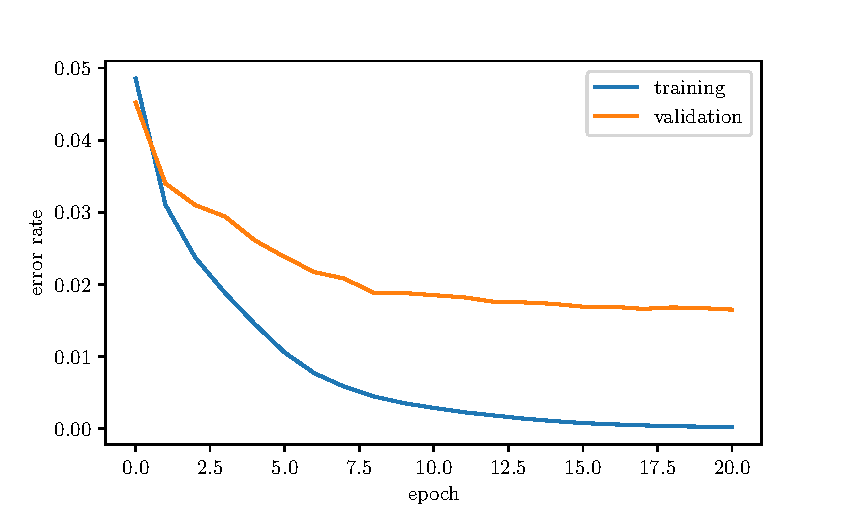
\includegraphics[width=0.6\textwidth]{assets/error_best.pdf}
  \caption{
    \label{fig:errorbest}
    Change of training and validation error while training epochs of MLP on full
    MNIST dataset. MLP has one hidden layer with 350 units and ReLu activation.
    Optimization with SGD used a learning rate of 0.02 and batches of 24 images.
  }
\end{figure}


\section{Regularization}\label{sec:regularization}

With the high amount of parameters (number of weight values), the MLP
is capable to express even complex functions.
This can lead to the problem of \emph{overfitting} which means the network
learns to express exactly the noisy training data instead of the general
underlying function. You see this generalization lack in \autoref{fig:errorbest}
as the gap between training and validation curves.
Regularization is an easy method to prevent overfitting by limiting the values
of the parameter vectors. Therefore I implemented
$L_1$ and $L_2$ regularization according to \cite{goodfellow71}.

$L_2$ regularization adds the squared sum of weights to the loss.
This means a large parameter values (huge square weight values) increase the loss a
lot and are therefore avoided. $L_1$ works similar but with the sum of absolute
parameter values. The amount of regularization can be controlled with the meta
parameter $\alpha$, which we did set to $\alpha=\frac{2}{\#\theta}$ in the lecture.

\begin{align}
  L_{L_2}(f_\theta, D) &= L(f_\theta, D) + \frac{\alpha}{2} \theta^T \theta,
  &\theta \leftarrow \theta - \epsilon (\alpha \theta + \Delta_\theta L(f_\theta,
  D)) \\
  L_{L_1}(f_\theta, D) &= L(f_\theta, D) + \alpha \lVert \theta \rVert,
  &\theta \leftarrow \theta - \epsilon (\alpha \mathop{sign}(\theta) + \Delta_\theta L(f_\theta,D))
\end{align}

You see in \autoref{fig:errorreg} that the regularization can prevent
overfitting like expected, validation and training error are very close.
Still also some draws of regularization are visible.
Both the train and the validation errors are higher with regularization.
Possibly this can be explained, by seeing the regularization update step also
as forgetting learned parameters.
In \autoref{fig:errorregl2} epochs 7 and 10 we see another incident,
probably also caused by the forgetting, the error rates jump up instead of descreasing.

\begin{figure}
  \centering
  \begin{subfigure}[b]{0.3\textwidth}
    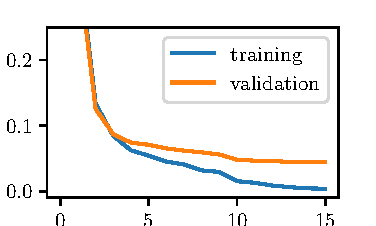
\includegraphics[width=\textwidth]{assets/error_noreg.pdf}
    \caption{none}
    \label{fig:errorregl1}
  \end{subfigure}
  \begin{subfigure}[b]{0.3\textwidth}
    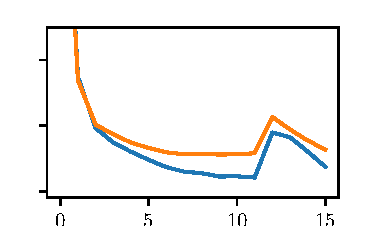
\includegraphics[width=\textwidth]{assets/error_l1.pdf}
    \caption{$L_1$ ($\alpha=0.0001$)}
    \label{fig:errorregl1}
  \end{subfigure}
  \begin{subfigure}[b]{0.3\textwidth}
    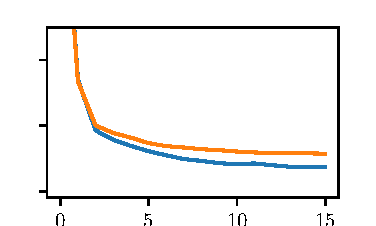
\includegraphics[width=\textwidth]{assets/error_l2.pdf}
    \caption{$L_2$  ($\alpha=0.005$)}
    \label{fig:errorregl2}
  \end{subfigure}
  \caption{Classification error while SGD training of MLP subset of MNIST without and with
    regularization. MLP has two hidden layers with each 100 units and ReLu activation.}\label{fig:errorreg}
\end{figure}



\begin{thebibliography}{99}
\bibitem{deeplearningorg}
  \url{http://deeplearning.net/tutorial/mlp.html}, last visit 2017/11/06
\bibitem{goodfellow71}
  I.\ Goodfellow, Y.\ Bengio, and A.\ Courville, \textit{Deep Learning, sec. 7.1},
  (MIT Press, 2016)
\end{thebibliography}

\end{document}
